Vélbúnaður prjónavélarinn er í grófum dráttum:  nálarbeðið, sleðinn/lásinn, litaskiptirinn og mótorinn.

\begin{figure}[H]
    \centering
    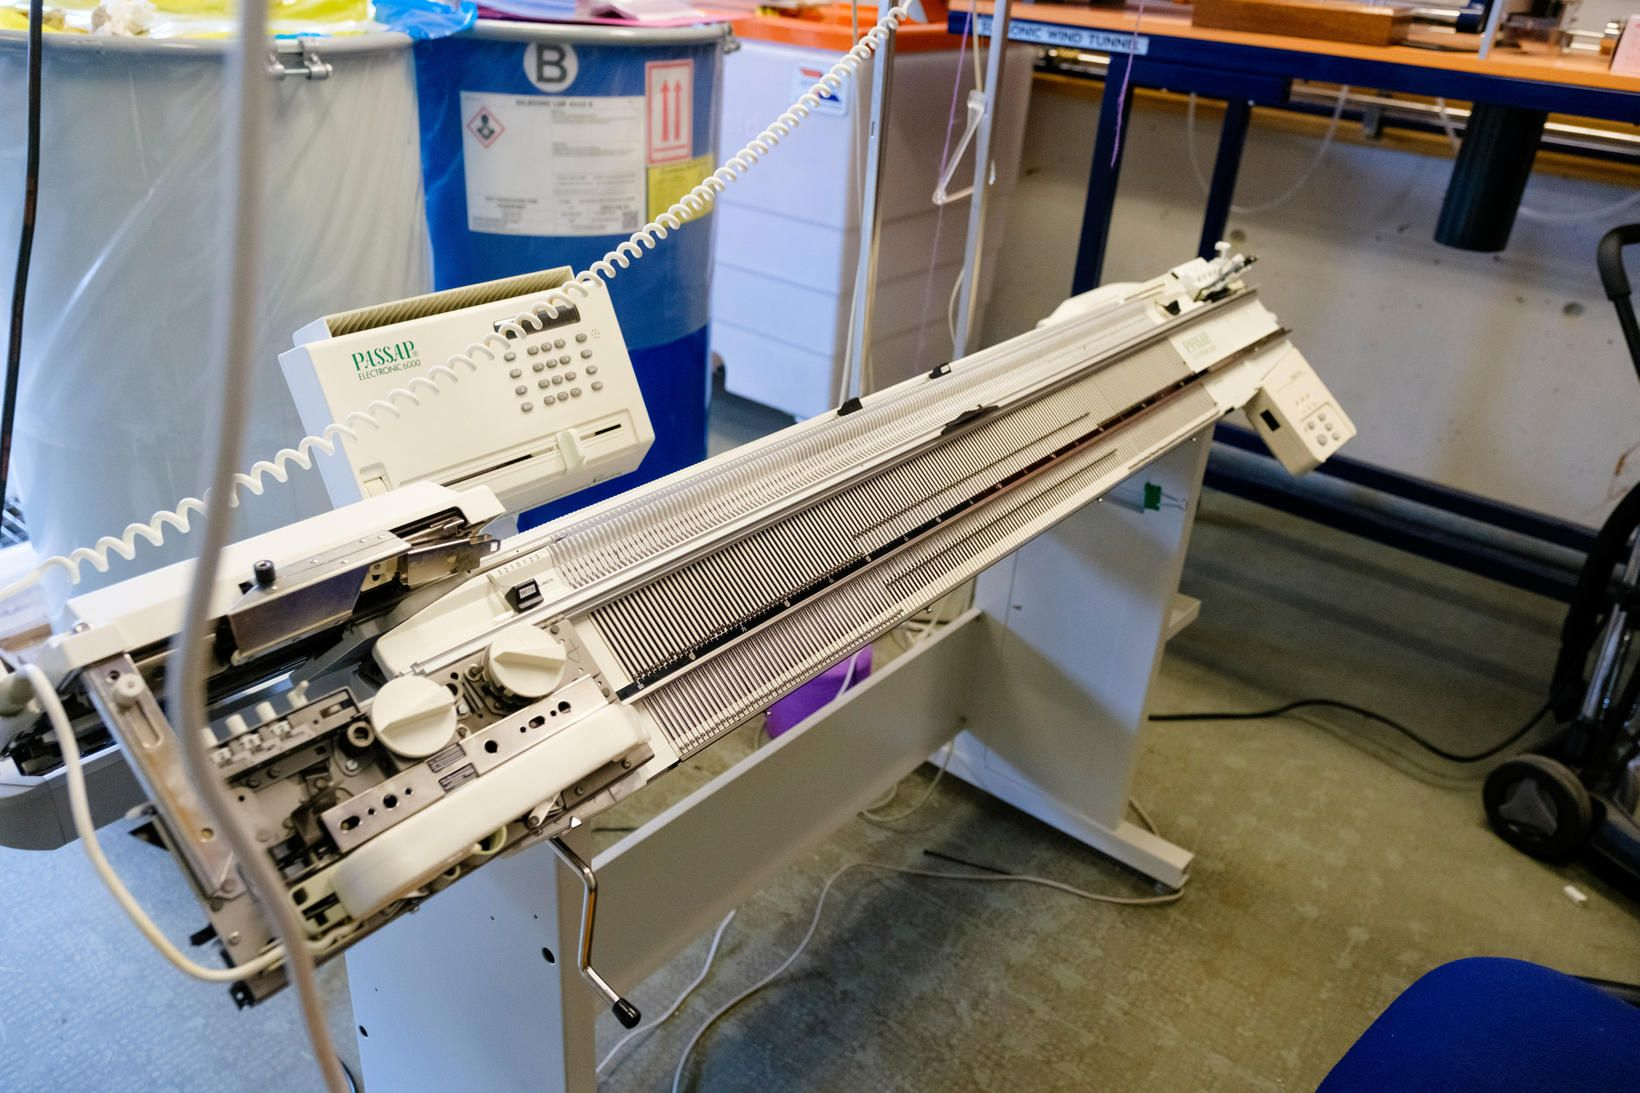
\includegraphics[width=0.5\linewidth]{myndir/elli/e6000.jpg}
    \caption{\textit{Passap E6000} prjónavél - \textit{mbl.is/Kristinn Magnússon}}
    \label{fig:e6000}
\end{figure}
\begin{enumerate}
    \item \textbf{Nálarbeðið inniheldur}
\begin{itemize}
    \item Braut sem sleðinn rennur eftir
    \item Nálastillara (e. pushers) sem eru undir nálunum í nálabeðinu og ýta nálunum í prjónastöðu. \\
    Þeir eru notaðir til að slökkva og kveikja á nálum fyrir hverja umferð, þ.e.a.s. setja nálar í óvirka eða virka stöðu.
    \item Nálarnar sem prjóna lykkjurnar ef þær eru í réttri stöðu þegar sleðinn fer yfir þær.
\end{itemize}
    \item \textbf{Sleðinn/lásinn samanstendur af}
    \begin{itemize}
        \item Tvo ljósaskynjara sem eru notaðir til að staðsetja sleðann á nálabeðinu.
        \item Tvo segla sem setja stöðu nálastillaranna fyrir næstu umferð.
        \item Braut sem fer með nálar í eftir tveimur mögulegum leiðum: 
        i) upp og prjónar lykkju í garninu eða ii) niður og prjónar ekki lykkju.
    \end{itemize}
    \item \textbf{Litaskiptirinn}
    \begin{itemize}
        \item Geymir garn.
        \item Er með einskonar takka sem sleðinn virkjar þegar hann fer yfir og skilar garni. Þá er nýtt garn sett í virka stöðu og það tekið upp á bakaleiðinni.
    \end{itemize}
    \item \textbf{Mótorinn} 
    \begin{itemize}
        \item Snýr belti sem hefur festingu fyrir sleðann.
        \item Festingin er með segul.
        \item Það eru þrír skynjarar á umgjörðinni sem inniheldur beltið sem skynja segulinn.
    \end{itemize}
\end{enumerate}
Hægt er að skipta vélbúnaðinum upp í tvö stýrikerfi. Annars vegar stýringinn á mótornum sem færir sleða lásinn frá vinstri til hægri yfir nálabeðið. Hinsvegar stýringinn á seglunum sem færa nálastillara á nálabeðinu upp og niður. Fyrir hvern nálastillir sem er stillt upp er lykkja prjónuð með garni fyrir þá nál í næstu umferð.
\subsubsection{Stýring nálarbeðs}
Upprunalega \textit{Passap E6000} vélin er með stjórnborð (svokölluð \textit{Form} tölva) sem er tengt með DIN-6 snúru við sleðann sem er læstur á nálabeðinu. Sleðinn er
með rafrás sem hefur ljósskynjara sem skynja göt á brautinni sem sleðinn rennur eftir. Götin eru \textit{2mm} breið og það eru \textit{3mm} á milli gata. Hver nál er \textit{5mm}. 

\begin{figure}
    \centering
\begin{tikzpicture}[auto, node distance=2cm, >=latex']

    % Define nodes
    \node [rectangle, draw, align=center] (sensor) {Ljósskynjari};
    \node [align=center, left=2cm of sensor] (light) {braut};
    \node [rectangle, draw, align=center, right=4cm of sensor] (sled) {Sleði/Lás};
    \node [rectangle, draw, align=center, above=3cm of sled] (console) {Stjórnborð};
    \node [rectangle, draw, align=center, below=3cm of sled] (magnets) {Seglar};
    \node [align=center, below=1.5cm of magnets] (needle) {nálstillir};
\draw[->] (light) edge[dotted, above] node{ljós} (sensor)
          (light) edge[dotted, below] node{skuggi} (sensor)
          (sensor) edge[above] node{hár straumur} (sled)
          (sensor) edge[below] node{lágur straumur} (sled)
          (sled) edge[->, dashed, right] node[rotate=-90, above] {hár straumur} (magnets)
          (sled) edge[->, dashed, left] node[rotate=-90, below] {lágur straumur} (magnets)
          (sled) edge[left] node[rotate=90, below] {lágur straumur} (console)
          (sled) edge[left] node[rotate=90, above] {hár straumur} (console)

          % Dashed line from console to sled coming out from the right side of the console with arrow only at the end
          (console.east) edge[bend left] node[rotate=-90, above] {hár straumur} (sled.east)
          (console.east) edge[bend left] node[rotate=-90, below] {lágur straumur} (sled.east)
          (magnets) edge[dotted] node[rotate=-90, above] {niður} (needle)
                    (magnets) edge[dotted] node[rotate=-90, below] {upp} (needle)
          ;
        \node[draw, rectangle, anchor=north west] at (0, 3) {
        \begin{tikzpicture}[x=1cm, y=0.8cm]
            \draw[thick] (0,0) -- (1,0) node[right] {5V};
            \draw[thick, dashed] (0,-0.5) -- (1,-0.5) node[right] {15V};
        \end{tikzpicture}
    };\end{tikzpicture}
    \caption{Stýring sem stillir nálar prjónavélarinar}
    \label{fig:original-pusher-control}
\end{figure}
Mynd \ref{fig:original-pusher-control} er kerfismynd af kerfinu sem stýrir nálastillurunum á nálabeðinu. Upprunalega stjórnborðinu var skipt út fyrir \textit{Arduino} með \textit{12v} spennubreyti sem er beintengdur við sleðann.
\begin{figure}
    \centering
    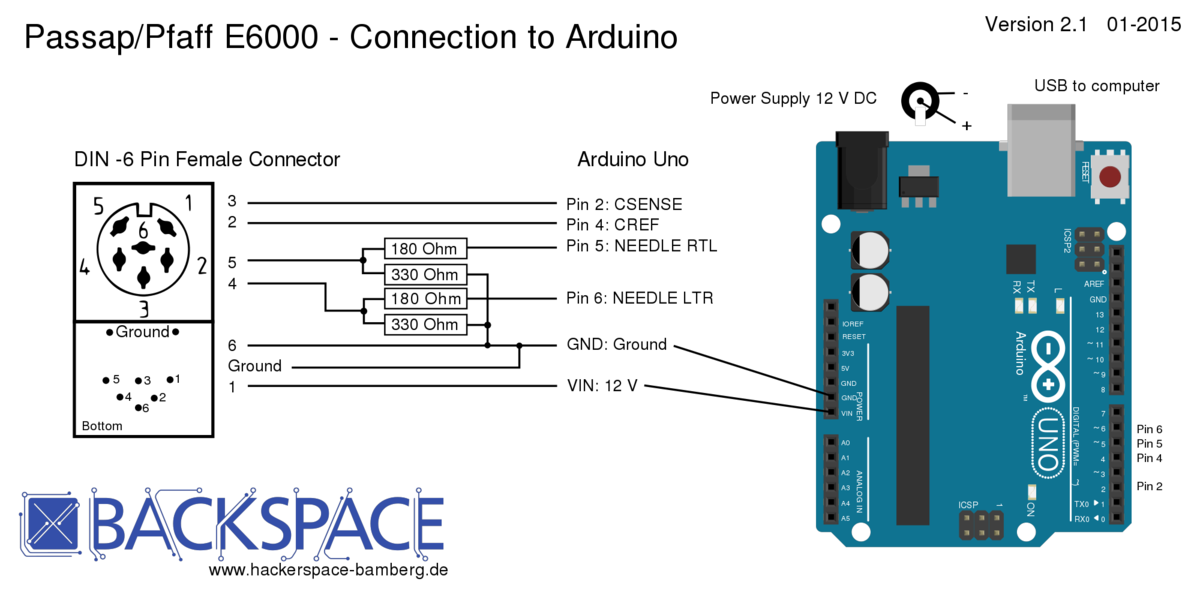
\includegraphics[width=0.75\linewidth]{myndir/bambergDIN6.png}
    \caption{Teikningar fyrir tengingu í gegnum DIN tengið voru fengnar af vefsíðu Bamberg \cite{bamberg}. }
    \label{fig:bambergDIN6}
\end{figure}
Pinnar 2 og 4 taka við straum frá ljósaskynjurum sleðans. Pinnar 5 og 6 stýra stöðu seglana tveggja. 
Það er einn segull fyrir hvorra áttina. Sleðinn stillir munstur fyrir næstu umferð á meðan hann fer yfir nálarbeðið og prjónar  munstrið sem er nú þegar á nálarbeðinu. Til að snúa við seglunum þarf að minnsta kosti \textit{12v} straum. Pinnarnir senda merki um það hvort straumnum sé hleypt á seglanna eða ekki. \textit{Arduino} er öflug örtölva og hefur þann kost að hún er með hraða og skilvikra innri klukku. Örtölvan getur því einbeitt sér að því að taka við merkjum um stöðu ljósskynjaranna. 
Í hvert skipti sem staðan á ljósskynjaranum sem er tengdur í pinna númer 2 á \textit{Arduino} borðinu breytist þá er staðan á á hinum skoðuð, sjá mynd \ref{fig:bambergDIN6}.

\begin{figure}
    \centering
    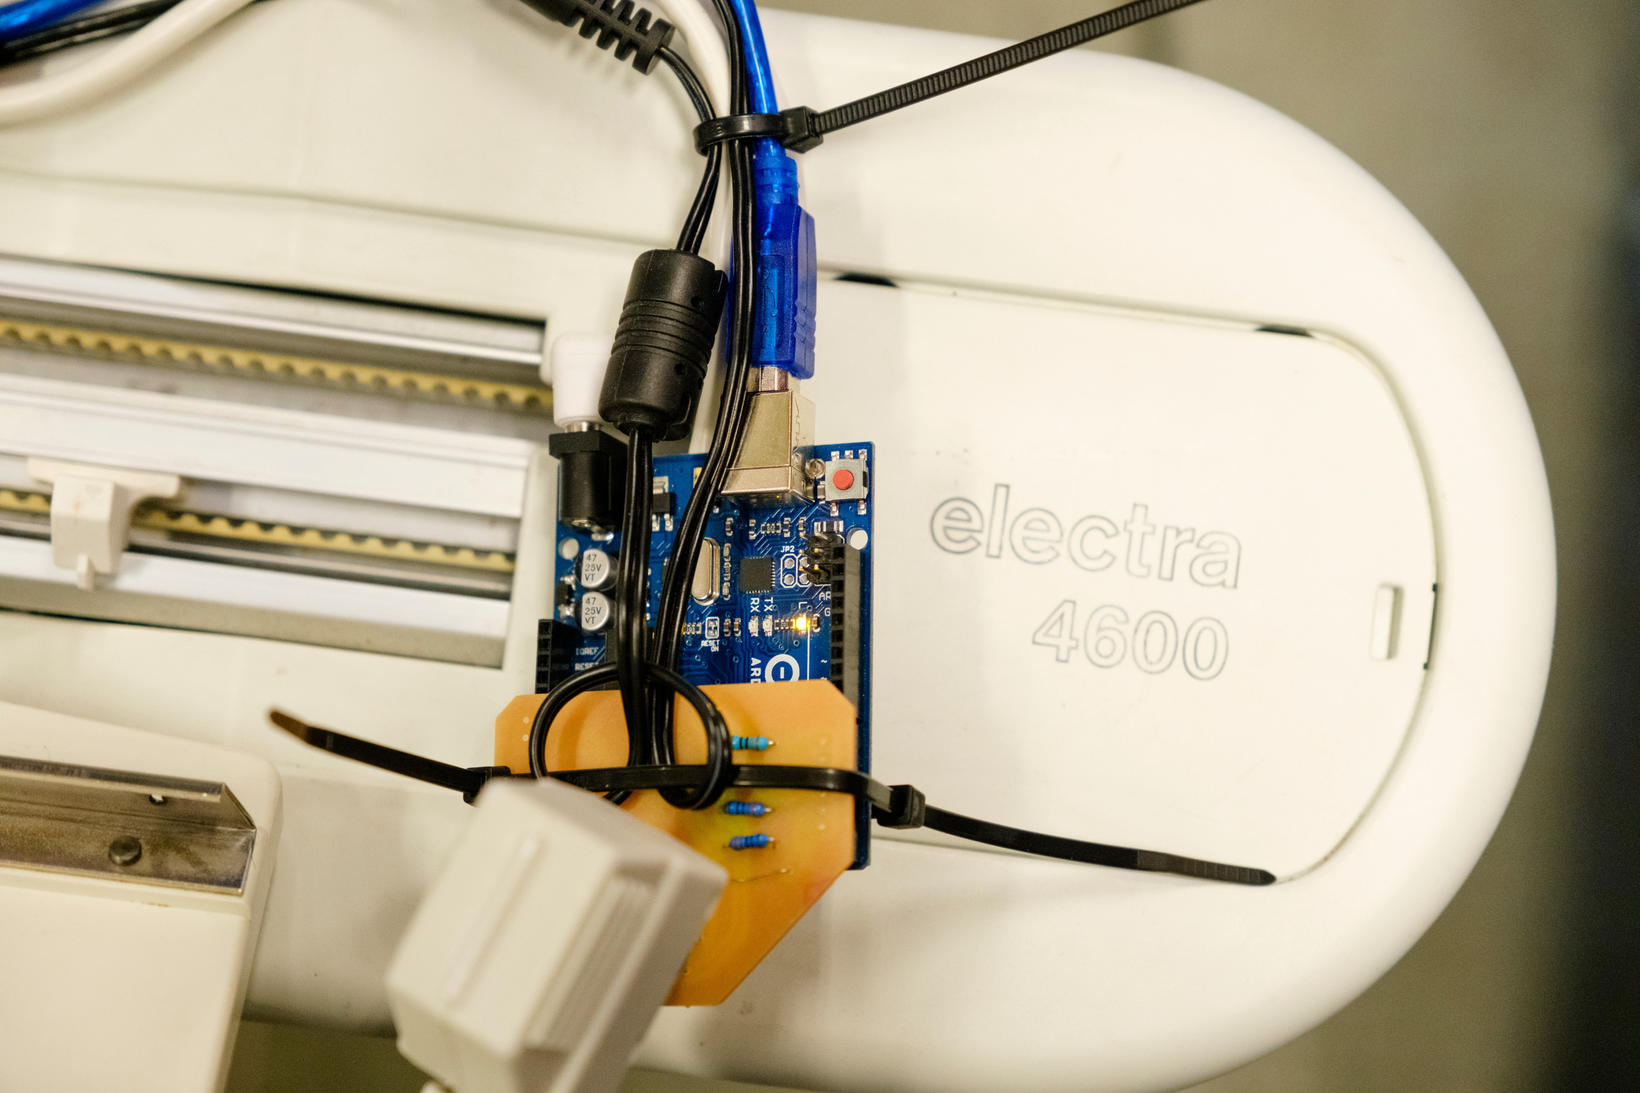
\includegraphics[width=0.5\linewidth]{myndir/elli/electra4600.jpg}
    \caption{\textit{Arduino} örtölva tengd við \textit{Passap E6000} - \textit{mbl.is/Kristinn Magnússon}}
    \label{fig:arduino}
\end{figure}
Það eru í raun tvö tilvik sem geta átt sér stað. Annaðhvort eru þeir í sömu stöðu eða í sitthvorri. Ef að aflestur ljósskynjara við breytingu á þeim sem er tendgur í pinna 2 er sú sama þá er við á leiðinni til hægri. Ef að þeir gefa sitthvort gildið þá erum við á leiðinni til vinstri. Örtölvan er því með innvortis teljara sem hækkar í gildi þegar aflesturinn er sá sami og lækkar þegar þeir gefa sitthvort gildið.
\begin{figure}[H]
    \centering
    \begin{tikzpicture}[auto, node distance=2cm, >=latex']
        \node [rectangle, draw, align=center] (Arduino) {\textit{Arduino} örtölva};
        \node [rectangle, draw, align=center, right=2cm of Arduino] (tölva) {tölva,nodejs};
        \node [rectangle, draw, align=center, below=4cm of Arduino] (sled) {Sleði/Lás};
        \node [below=1cm of sled] (magnets) {};
        \draw[-] (sled) edge[dashed, right] node[rotate=-90, above] {} (magnets);
        
    \end{tikzpicture}
    \caption{Caption}
    \label{fig:enter-label}
\end{figure}
!!! vantar texta um serial uppsetningu og svoframvegis\\

Stýringin er uppsett þannig að örtölvan ítrar stanslaust í gegnum segð sem athugar hvort það hafi verið send einhver skilaboð yfir serial samskipti á USB snúrunni. Í hvert skipti sem ljósskynjarinn breytir um gildi er sú ítrun trufluð og teljarinn hækkaður eða lækkaður eftir því í hvort við séum að fara til hægri eða vinstri. Ef að það eru skilaboð þá sækir hann úr því streng sem inniheldur línuvigur úr fylkinu,\\
sendir \texttt{r} og \texttt{l} til að fá nýjan, ég klára á morgun
\subsubsection{Stýring á mótor}
fjallað um breytingar\\ 
!! ég er ekki búin, klára á morgun ég lofa
\subsubsection{Opið vefviðmót}
